\chapter{Implementation}
\label{sec:impl}
Reviewernet is a fully client-side application. It builds on a bibliographic dataset extracted from a reference corpus containing more than 180 million records.

The goal is to facilitate a complex process, as the reviewer selection, through multiple and coordinated views about papers and researchers.

In this chapter, we describe our implementation choices, namely: the data and the preprocessing phase, languages, frameworks and external libraries used to deploy the user interface, concluding with an analysis of the code that implements additional features of our interactive visualization system.
\section{The Data}
To construct the reference dataset, we collected papers, authors and citations from eight selected sources in the field of Computer Graphics, taken from the Semantic Scholar Research Corpus \cite{ammar:18}. 

The original corpus currently contains more than 180 millions research papers published in all fields, provided as a set of gzipped JSON archives. In Figure \ref{jsonfields} there is the full list of the attributes of a generic record that represents a pubblication.

\begin{figure}[!ht]
    \centering
    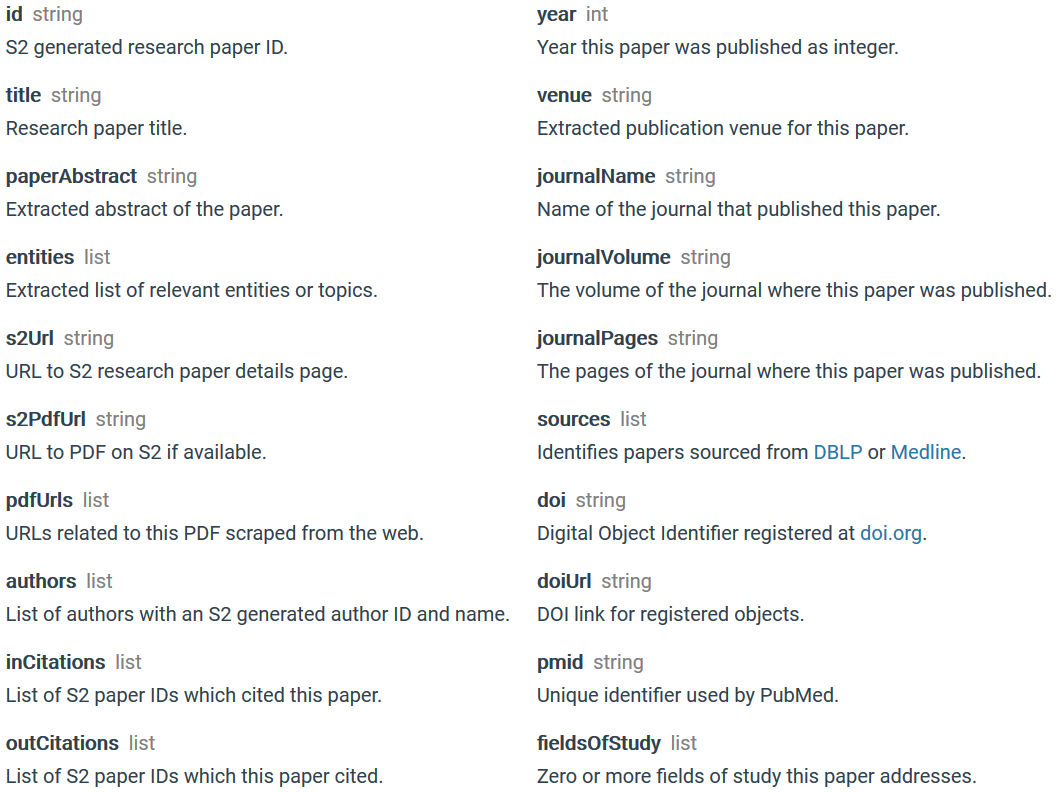
\includegraphics[height=10cm]{fig/corpusfields.png}
    \caption{Definition of attributes of the Semantic Scholar coprus.\label{jsonfields}}
\end{figure}

To keep complexity low and offer a cleaner visualization, we filtered the corpus extracting only publications from journals and conference proceedings listed in Table \ref{table:sources}, spanning the years in-between 1995 and 2019. 

The final reference dataset contains 22.887 papers, 145.900 citations, and 29.549 authors.
\begin{table}[!h]
\renewcommand{\arraystretch}{1.3}
\centering
\begin{tabular}{|l|c|}
\hline
ACM Transactions on Graphics & 2594\\ 
Computer Graphics and Applications  & 1697 \\ 
Computer Graphics Forum & 3521\\ 
Computers \& Graphics & 2092\\ 
IEEE Transactions on Visualization and Computer Graphics & 3638\\ 
Visual Computer & 2107\\ 
Proceedings of IEEE Conference Visualization (pre 2006) & 474 \\ 
Proceedings of ACM SIGGRAPH (pre 2003) & 6718\\
\hline
\end{tabular}
\caption{The selected sources from the Semantic Scholar Research Corpus used in our demonstration scenario. The final reference dataset contains 22.887 papers, 145.900 citations, and 29.549 authors.}
\label{table:sources}
\end{table}

%\input{stats.tex}
\subsection*{Pre-Processing}
\label{sec:preproc}

pre-proc is crucial: we want to lower data complexity, while maintaning choerence and topic coverage to properly support the reviewer selection process. After non-paper and useless attributes deletion, each partition parsed and filtered separatedly by a python script. Then consolidation step 
\begin{itemize}
    \item check citations consistency
    \item merge data obtaining 3 files that represent the Computer Graphic reference corpus. (descrivo i tre file con attributi)
\end{itemize}

\section{Languages \& External Libraries}
\label{sec:lang}
\begin{itemize}
    \item static UI: HTML5, CSS3, bootstrap
    \item dynamic: JS (JqueryUI for widgets) and D3JS
    \item preproc: Bash and Python (fuzzywuzzy) 
\end{itemize}

\section{Additional features}
\label{sec:misccode}

\begin{itemize}
    \item export/load session snapshot (formato file, spiegare inconsistenza fra id di varie versioni del corpus)
    \item import from biblio \& \texttt{p\_search}
    \item generating a custom reviewernet instance
\end{itemize}